\documentclass[tikz]{standalone}
\usepackage{tikz}
\usepackage{circuitikz}

\begin{document}
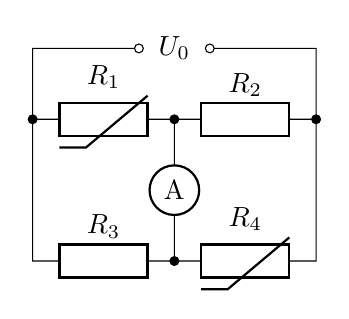
\begin{tikzpicture}[european, scale=0.9]
	\draw (1.5,0) to [short, o-] (0,0) -- (0,-3) to [R, l=$R_3$] (2,-3) to [thR, l=$R_4$] (4,-3) -- (4,0)  to [short, -o] (2.5,0)
	(0,-1) to [thR, l=$R_1$, *-] (2,-1) to [R, l=$R_2$] (4,-1) to [short, -*] (4,-1)
	(2,-1) to [short, *-] (2,-1.65) (2,-2.35) to [short, -*] (2,-3) 
	(2,0) node[]{$U_0$};
	\draw [thick, fill = white] (2,-2) circle (0.35);
	\node at (2,-2) {A};
\end{tikzpicture}
\end{document}
